Introduction to \textbf{anisotropic} transport phenomenon.
\subsection{Theory basics}
\subsubsection{Quadrik}
 Every symmetric 2nd rank tensor can be presented as an ellipsoid in the three dimensional space
 
\begin{multicols}{3}
		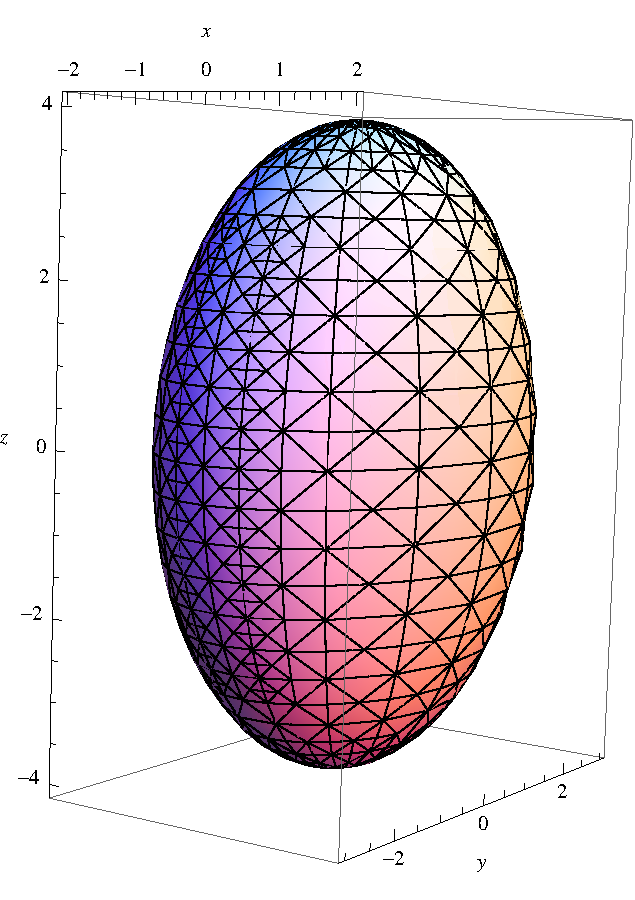
\includegraphics[scale=0.2]{images/ellipsoid.pdf}
	\columnbreak	
		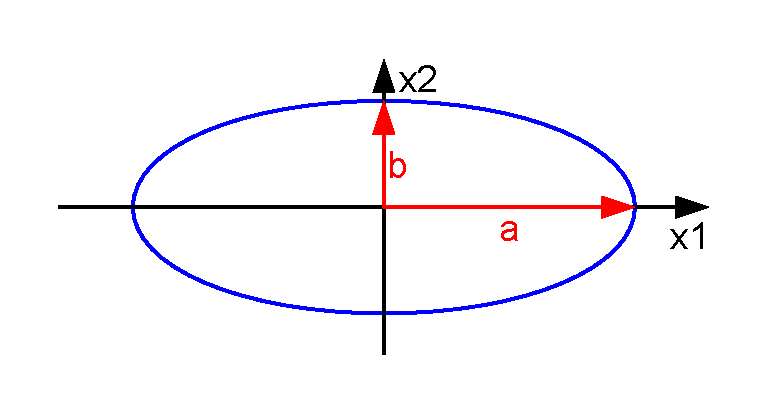
\includegraphics[scale=0.4]{images/quadrik_2d_ellipse.pdf}
\columnbreak
$$
	\sigma_{ij}=\begin{pmatrix}
		\sigma_1 & 0 & 0 \\
		0 & \sigma_2 & 0 \\
		0 & 0 & \sigma_3 \\
	\end{pmatrix}
$$
	$$\sigma_1x_1^2+\sigma_2x_2^2+\sigma_3x_3^2=1$$
	$$
	a=\frac{1}{\sqrt{\sigma_1}}; b=\frac{1}{\sqrt{\sigma_2}};
	c=\frac{1}{\sqrt{\sigma_3}}
	$$
\end{multicols}
\renewcommand{\arraystretch}{1.8}	

\begin{tabularx}{\columnwidth}{XXXX}
	\hline 
	field & law & quadric (only symmetric) & notes\\
	\hline 
	Thermal conduction &
	$j_i= -\lambda_{ij}\dfrac{\partial T}{\partial x_j} $ &
	$\lambda_1 x_1^2+\lambda_2 x_2^2+\lambda_3 x_3^2=1$ &
	$\lambda_{ij}$: therm. conductivity tensor $\lambda_{ij} = \lambda_{ji}$\newline $\rho_{ij}$: therm. resistivity tensor, $\rho_i = \dfrac{1}{\lambda_i}$\\
	
	
	\textbf{Spec Case: Heat Flow across a flow plate}&
	$\frac{\partial T}{\partial x_2}=0$ $\frac{\partial T}{\partial x_3}=0$ &	
	$
	\lambda_{11}= \lambda_1=\dfrac{j_1}{\partial T/ \partial x_1}
	$&
	temp. gradient parallel to $x_1$\\


	\textbf{Spec. case: Heat flow down a long rod(stab)} &
	$\frac{\partial T}{\partial x_1}=\rho_{11}j_1$\newline$ \frac{\partial T}{\partial x_2}=\rho_{12}j_1$\newline$ \frac{\partial T}{\partial x_3}=\rho_{13}j_1$&
	& it is recommended to work with the therm. resistance $\rho$ \\
	\hline 
	Electrical conduction & $j_i=-\sigma_{ij}\dfrac{\partial \phi}{\partial x_j}=\sigma_{ij}E_j$ \newline $j_i = \dfrac{1}{\rho_{ij}}E_i$&
	&
	$\sigma_{ij}$: electrical conductivity tensor\newline $\rho_{ij}$: electrical resistivity tensor \\
	\hline 
	Diffusion & $j_i=-D_{ij}\frac{\partial c}{\partial x_j}$&
	&
	$D_{ij}$: Diffusion tensor\\
	\hline 
\end{tabularx}
\renewcommand{\arraystretch}{1.2}	
